
% Converted from: Physical properties.pdf (handwritten notes)
\documentclass[11pt,a4paper]{article}
\usepackage{notes}
\usepackage{graphicx}
\usetikzlibrary{arrows.meta}

\title{Physical Properties of Rocks and How We Estimate Them}
\author{Derrick Hasterok}
\date{\today}

\begin{document}
\maketitle

\section{Introduction}
In geophysics we typically \emph{measure fields} and \emph{infer properties}, the reverse of many classical physics problems. Rock properties arise from minerals and the fluids in pore space and depend on the \emph{state} of the system (pressure, temperature, volume, composition).

\subsection{State variables}
\begin{itemize}
  \item Pressure $P$ (Pa, MPa, GPa, kbar). Note: $1\,\mathrm{kbar} \approx 100\,\mathrm{MPa}$.
  \item Temperature $T$ (K or $\degC$). Absolute scale: not ``degrees K''; conversion: $T_{\mathrm{K}} = T_{\degC} + 273.15$.
  \item Volume $V$ (m$^3$ or km$^3$).
  \item Composition (moles, wt\%, ppm, fractions). Can refer to phase modes or elemental/oxide concentrations.
\end{itemize}

\section{Key Physical Properties}
\begin{itemize}
  \item Density: $\rho = m/V$ (kg\,m$^{-3}$).
  \item Thermal expansivity (volumetric, at $P$ const.): $\alpha$ (K$^{-1}$).
  \item Compressibility $\beta_T$ and bulk moduli $K_T=1/\beta_T$, $K_S$ (MPa, GPa).
  \item Shear modulus $\mu$ (MPa, GPa).
  \item Seismic velocities: $v_p$ (compressional), $v_s$ (shear) (m\,s$^{-1}$ or km\,s$^{-1}$).
  \item Thermal conductivity $k$ (W\,m$^{-1}$\,K$^{-1}$); heat capacity $c_p$ (J\,kg$^{-1}$\,K$^{-1}$).
  \item Thermal diffusivity $\kappa = k/(\rho c_p)$ (mm$^2$\,s$^{-1}$ or km$^2$\,Ma$^{-1}$).
  \item Heat production $A$ (W\,m$^{-3}$ or $\mu$W\,m$^{-3}$), or $H$ (W\,kg$^{-1}$).
\end{itemize}

\section{Strategies to Estimate Properties}
\subsection{Direct measurements}
\begin{itemize}
  \item Lab or in situ; strong control on state; targeted protocols.
  \item Consider scaling, representativeness, cost, and sampling.
\end{itemize}

\subsection{From composition}
\begin{itemize}
  \item From mineral modes: simple to apply when modes known; extrapolation outside calibrations is risky (??).
  \item From major elements: widely available; captures broad trends but may obscure mineral-control (assumptions needed).
  \item Thermodynamics: internally consistent; works with or without known modes; computationally intensive and specialized.
\end{itemize}

\subsection{Indirect correlations}
\begin{itemize}
  \item Property--property regressions (e.g., $v_p$ vs $\rho$); rapid domain mapping but potentially non-unique.
  \item Data-driven/ML: handles large, multivariate datasets; may be biased by training data and limited in state extrapolation.
\end{itemize}

\section{Examples and Figures from Notes}

\subsection{Density from composition}
An empirical relation for many silicates (Group~I) is suggested as
\begin{equation}
  \rho\;[\mathrm{kg\,m^{-3}}] \;=\; 2532 + 216\,\mathrm{Fe} + 608\,M\; - 10\,\mathrm{MALI}, \quad \text{(notation as in notes; confirm definitions: ??)}
\end{equation}
where Fe is an iron number (wt\%), $M$ a maficity parameter, and MALI is the modified alkali--lime index (precise definitions deferred: ??).
\begin{figure}[h]
  \centering
  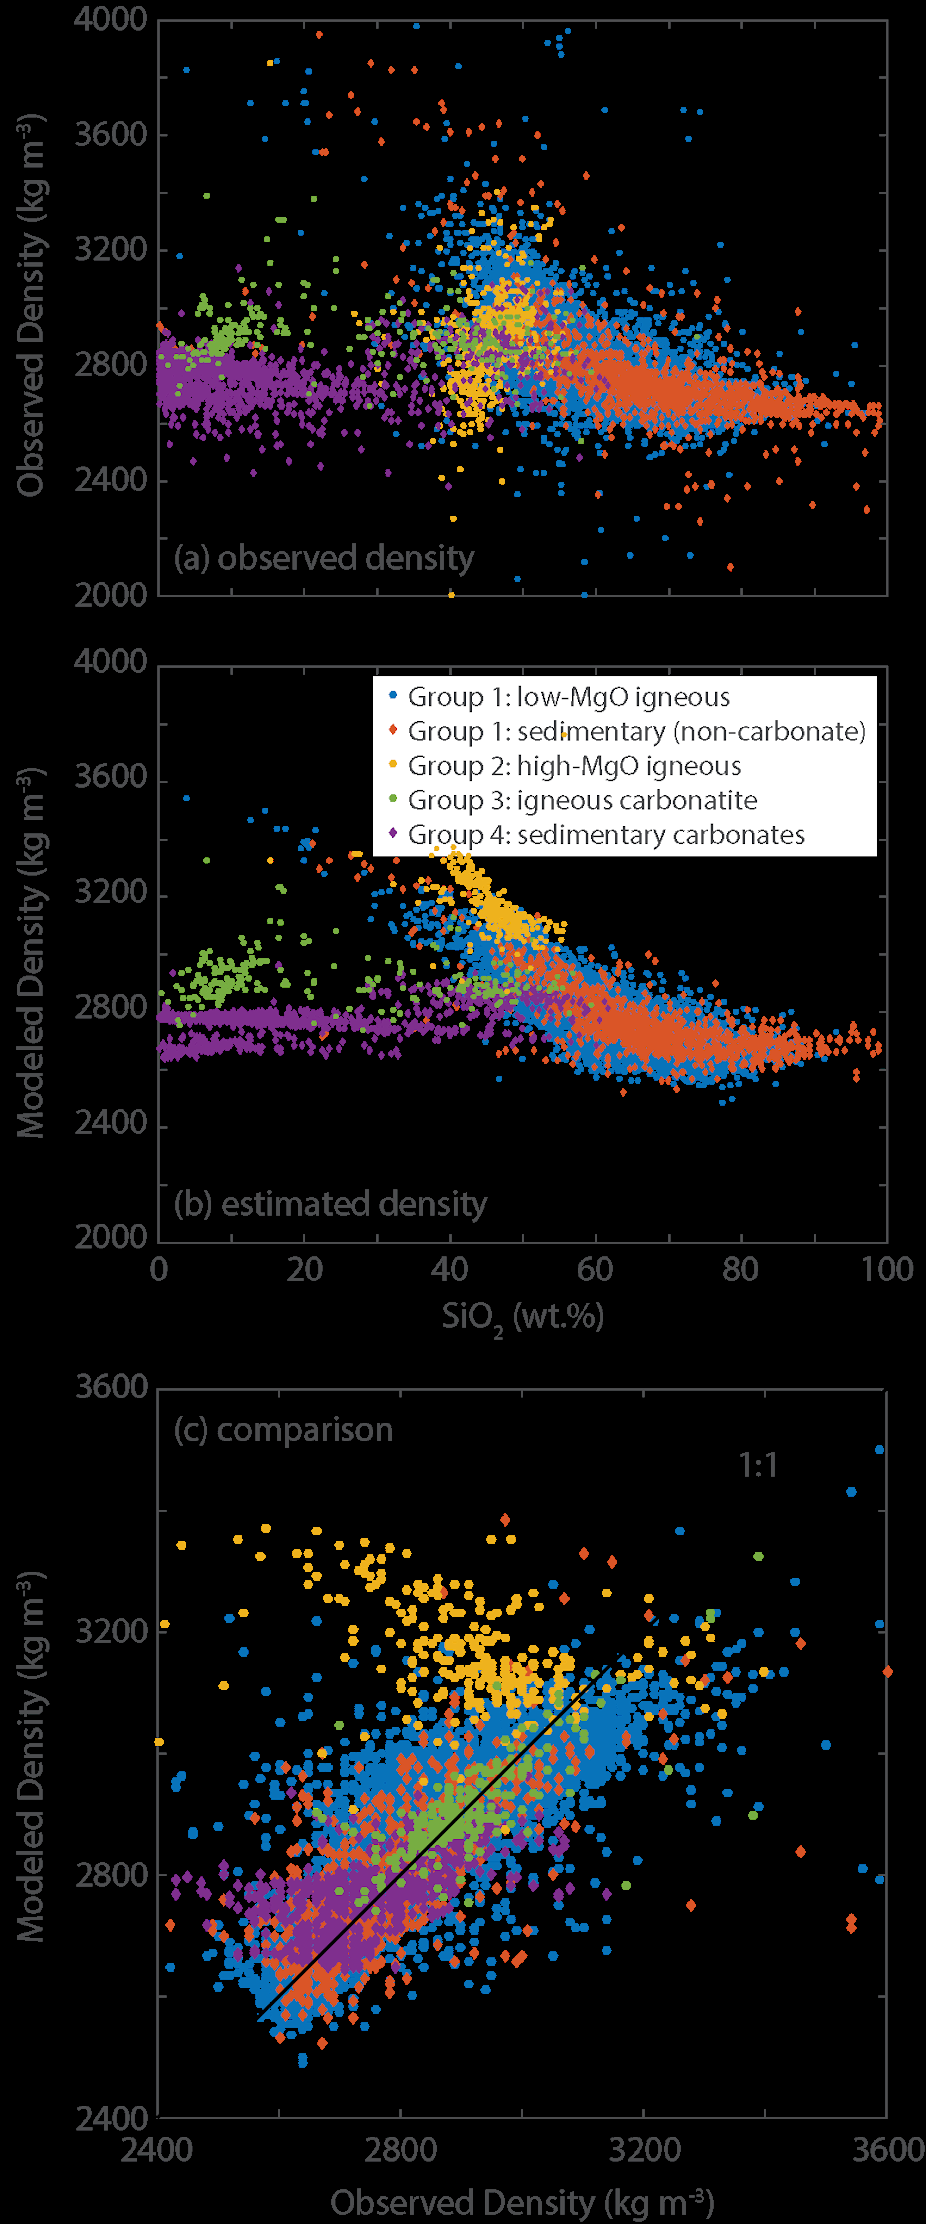
\includegraphics[width=0.8\linewidth]{extracted_images/Physical_properties_p8_img57.png}
  \caption{Density vs composition (extracted from notes).}
\end{figure}

\subsection{Other property trends}
Several properties co-vary with composition or with each other (e.g., thermal conductivity with composition; weakly with $v_p$), enabling indirect estimates.

\begin{figure}[h]
  \centering
  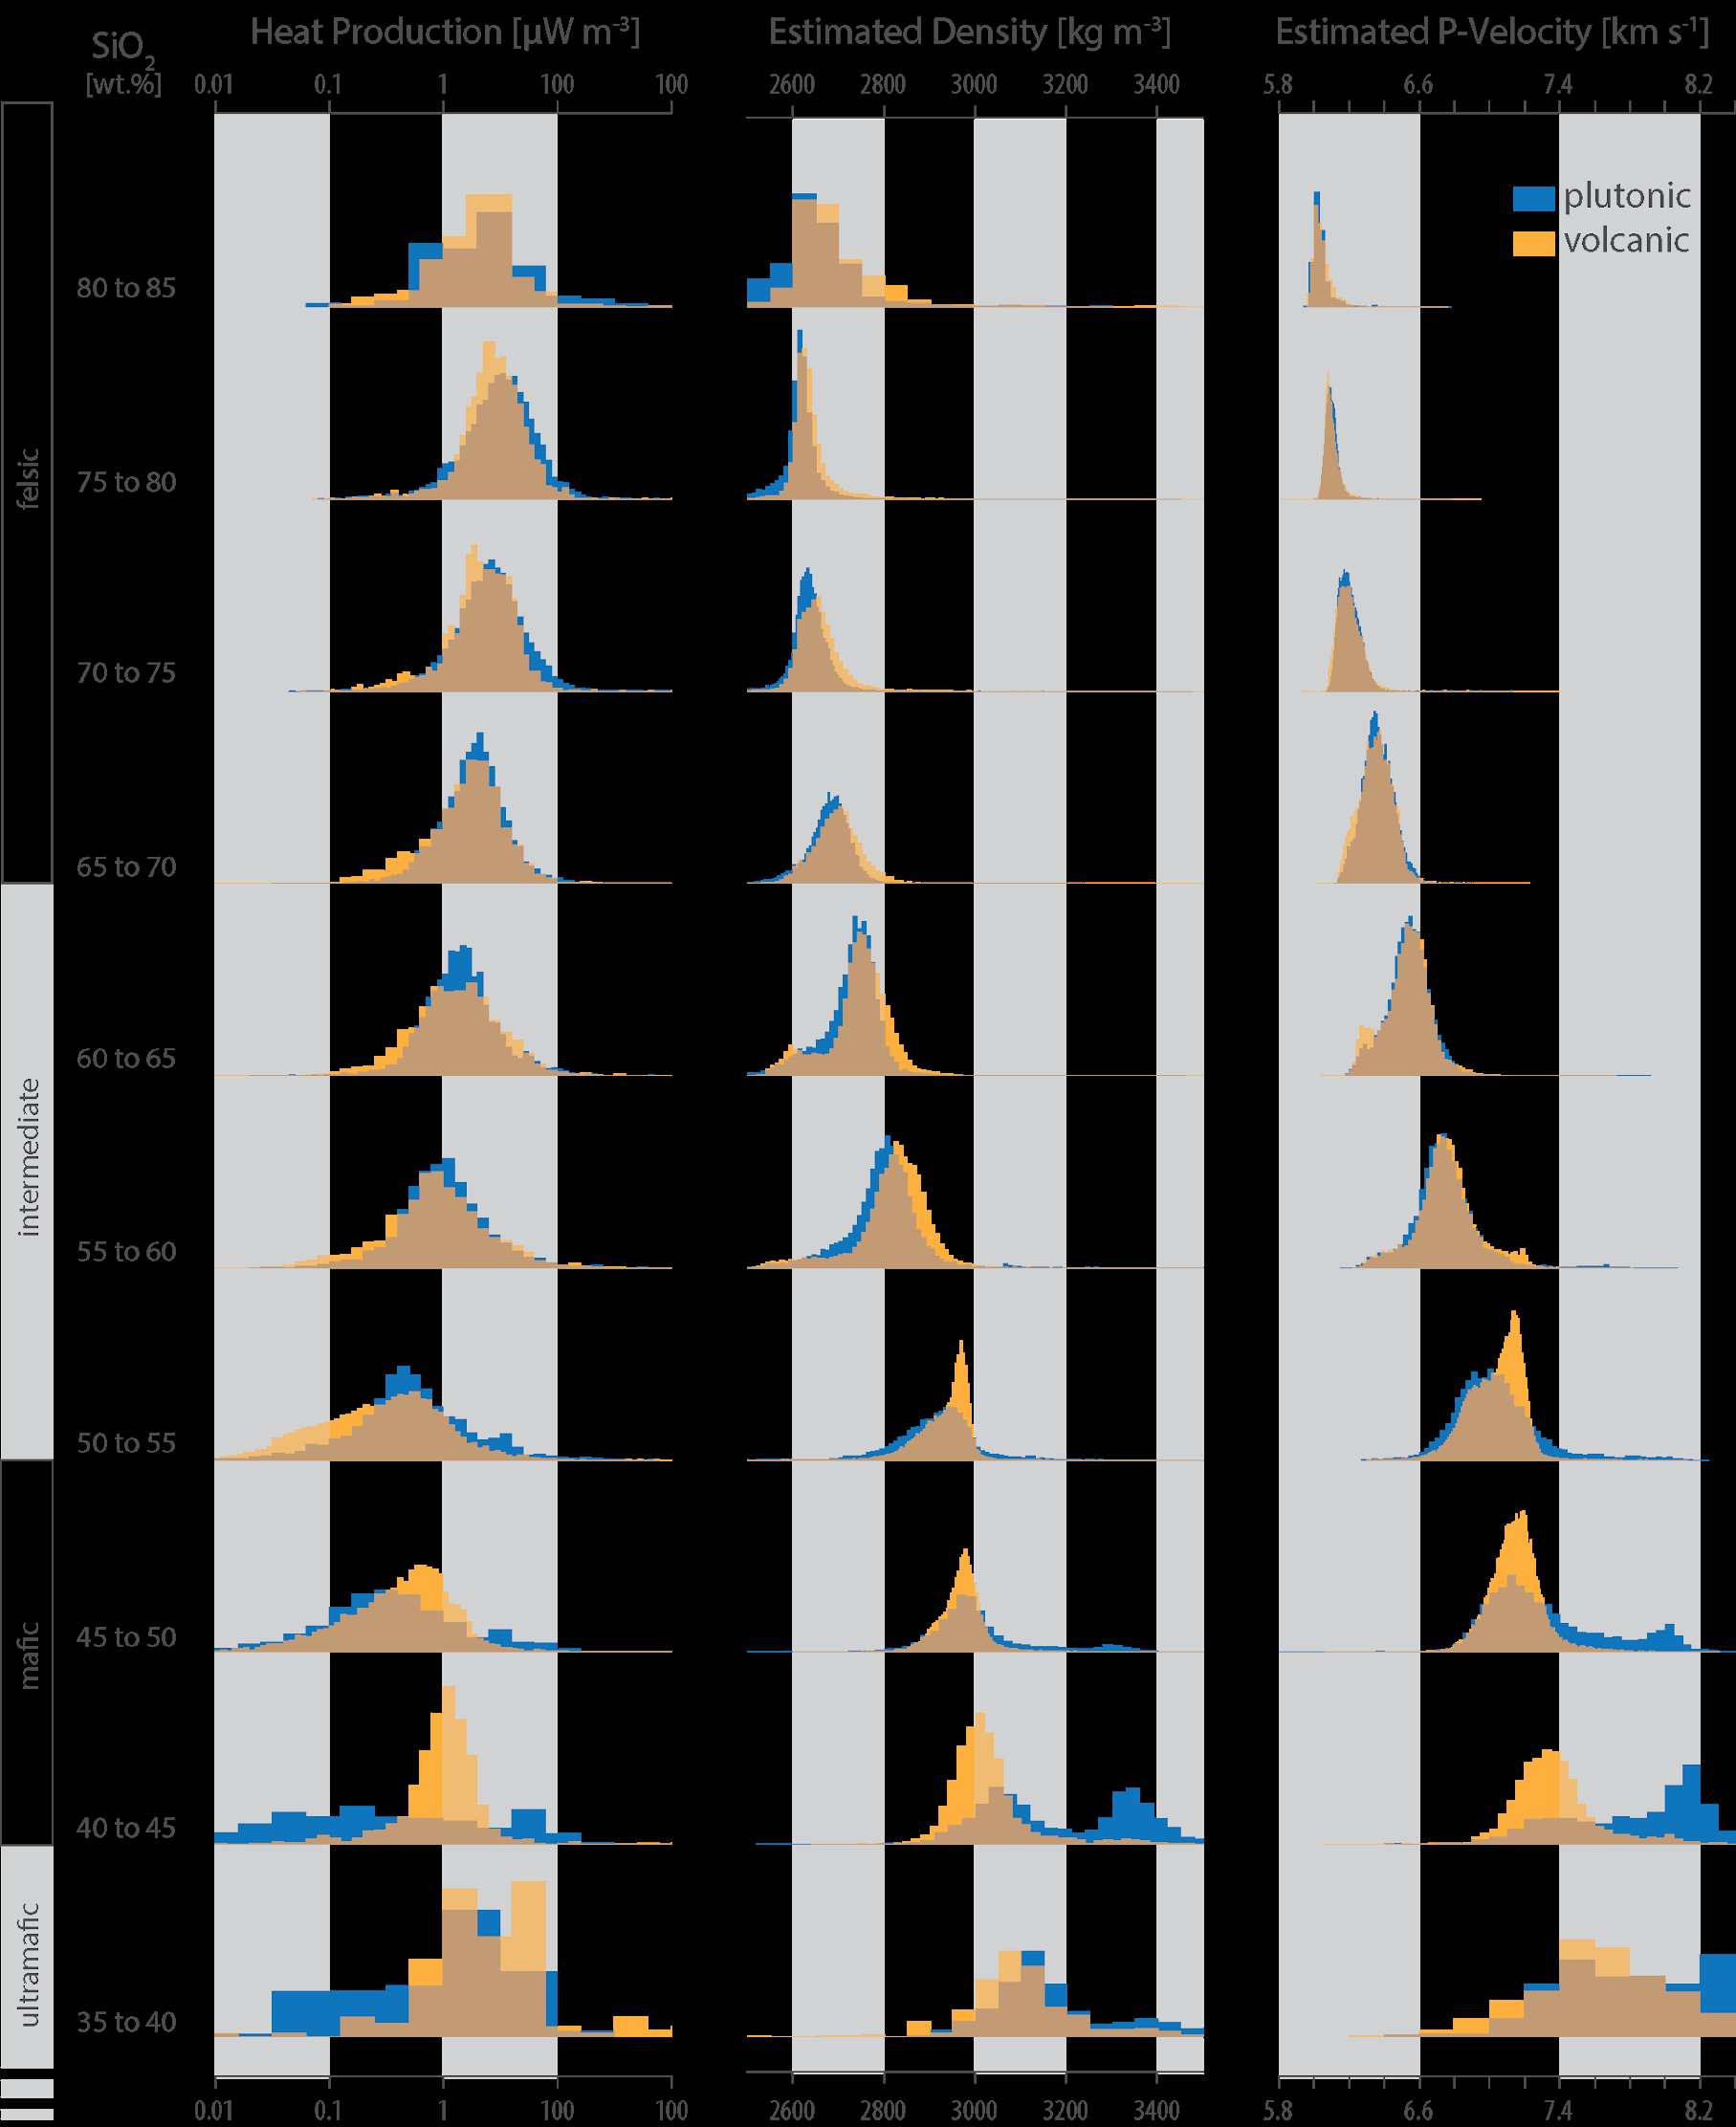
\includegraphics[width=0.8\linewidth]{extracted_images/Physical_properties_p9_img66.png}
  \caption{Compositional trends among properties (extracted from notes).}
\end{figure}

\begin{figure}[h]
  \centering
  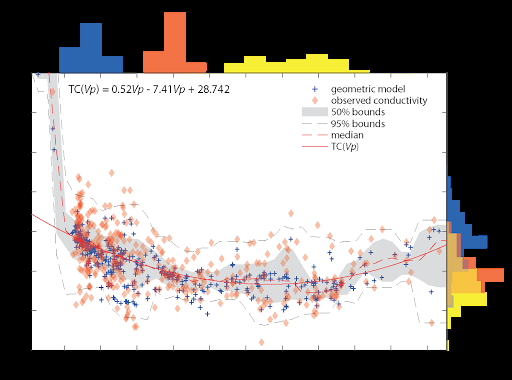
\includegraphics[width=0.8\linewidth]{extracted_images/Physical_properties_p10_img71.png}
  \caption{Thermal conductivity vs composition or $v_p$ (extracted from notes).}
\end{figure}

\begin{figure}[h]
  \centering
  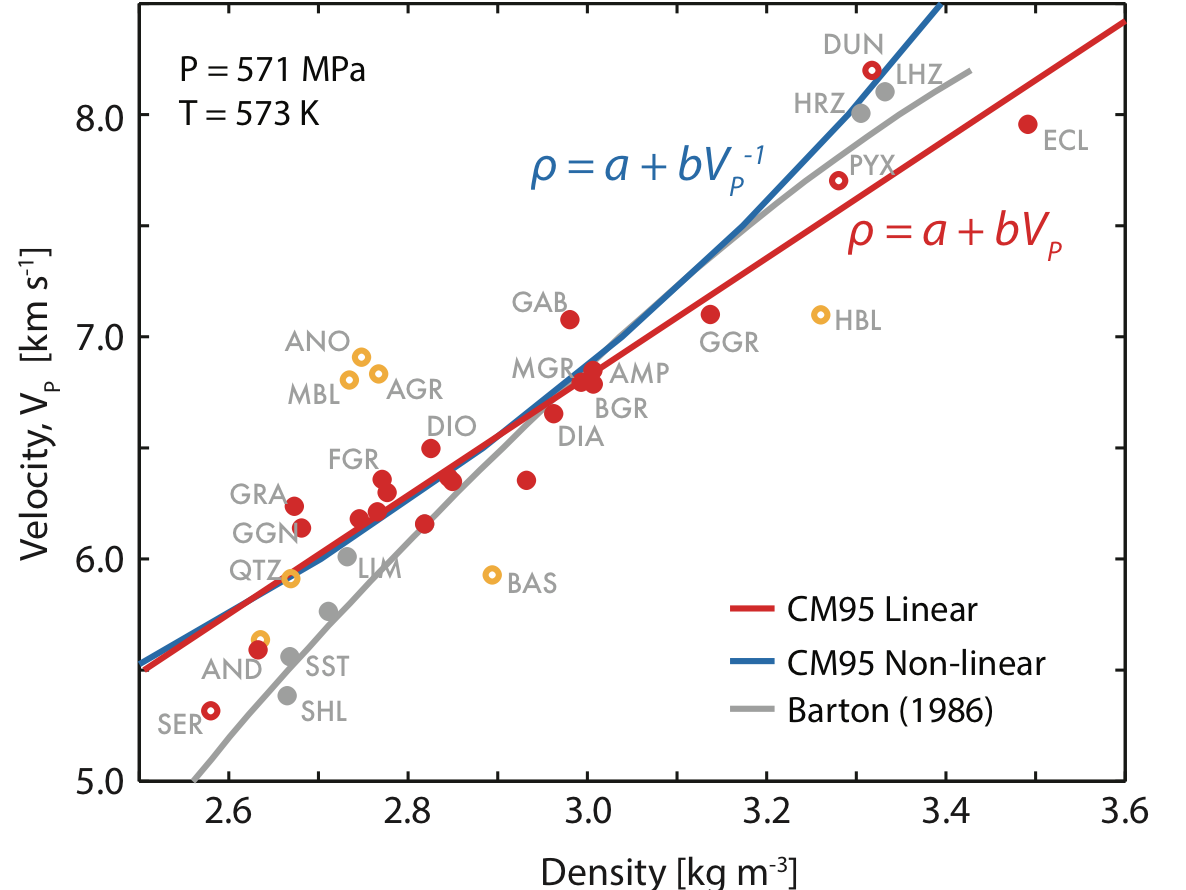
\includegraphics[width=0.8\linewidth]{extracted_images/Physical_properties_p11_img76.png}
  \caption{Seismic velocity vs density as composition proxy (extracted from notes).}
\end{figure}

\section{Pressure, Temperature, and Porosity Effects}
For a given rock, three principal factors influence velocity:
\begin{itemize}
  \item Pressure increases close cracks and stiffens the frame $\Rightarrow$ $v$ increases.
  \item Temperature increases reduce density and moduli $\Rightarrow$ $v$ decreases.
  \item Porosity/fractures impede wave paths $\Rightarrow$ lower apparent $v$ (in crystalline rocks, density reduction may be minor).
\end{itemize}

\begin{figure}[h]
  \centering
  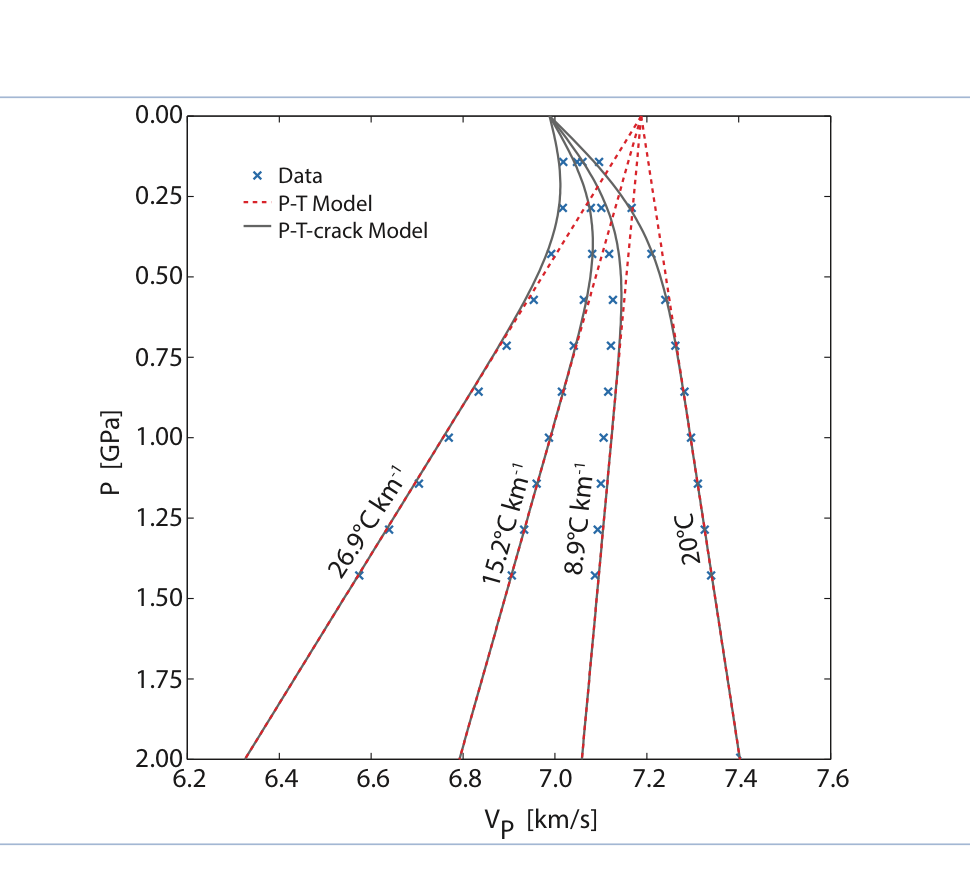
\includegraphics[width=0.8\linewidth]{extracted_images/Physical_properties_p12_img80.png}
  \caption{Velocity trends with P and T (extracted from notes).}
\end{figure}

\begin{figure}[h]
  \centering
  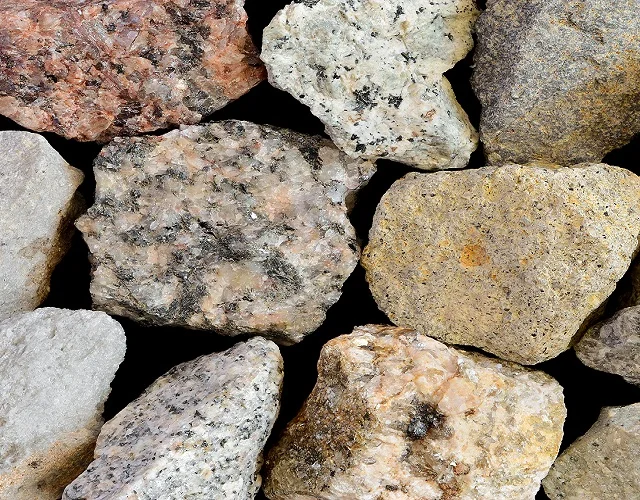
\includegraphics[width=0.8\linewidth]{extracted_images/Physical_properties_p13_img85.png}
  \caption{Effect of porosity/fractures on velocity (extracted from notes).}
\end{figure}

\section{Mixing Relations}
Rocks are mixtures; bulk properties require mixing laws.

\subsection{Common means}
\begin{itemize}
  \item Arithmetic mean (e.g., density, some heat capacities): $X = \sum_i w_i X_i$.
  \item Geometric mean (random mixtures; often used for conductivity): $\displaystyle X = \prod_i X_i^{\,w_i}$.
  \item Harmonic mean (series layers; transport-limited): $\displaystyle X = \left(\sum_i \frac{w_i}{X_i}\right)^{-1}$.
\end{itemize}

\subsection{Voigt--Reuss--Hill (VRH)}
For elastic moduli/velocities: $X_V$ (arithmetic), $X_R$ (harmonic), and Hill average $X_{\mathrm{VRH}} = \tfrac12(X_V+X_R)$.

\subsection{Isotropy vs anisotropy}
\begin{itemize}
  \item Isotropic properties (e.g., density) are direction independent.
  \item Anisotropic properties (e.g., thermal/electrical conductivity, elastic moduli) vary with direction.
\end{itemize}

\paragraph{Bulk density as an example.} With volume fractions $f_i$ and constituent densities $\rho_i$,
\begin{equation}
  \rho_{\mathrm{bulk}} = \sum_i f_i\,\rho_i .
\end{equation}

\begin{figure}[h]
  \centering
  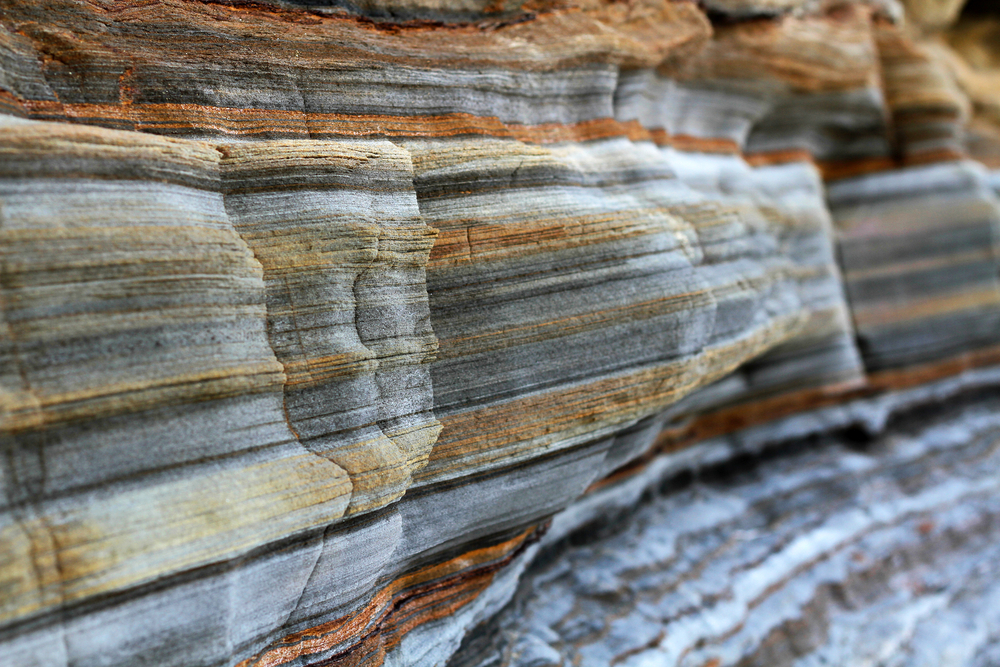
\includegraphics[width=0.8\linewidth]{extracted_images/Physical_properties_p13_img86.png}
  \caption{Additional schematic/plot related to mixing or trends (extracted from notes).}
\end{figure}

\bigskip

oindent\textit{Transcription notes:} Ambiguities in the handwriting/OCR are marked with ``??'' to flag items needing your confirmation.

\end{document}
